\section{LNA Architecture}

In this section, we present the architecture of the Low Noise Amplifier (LNA) designed, the complete architecture is shown in Figure \ref{fig:schem-lna}. 

\begin{figure}[H]
    \centering
    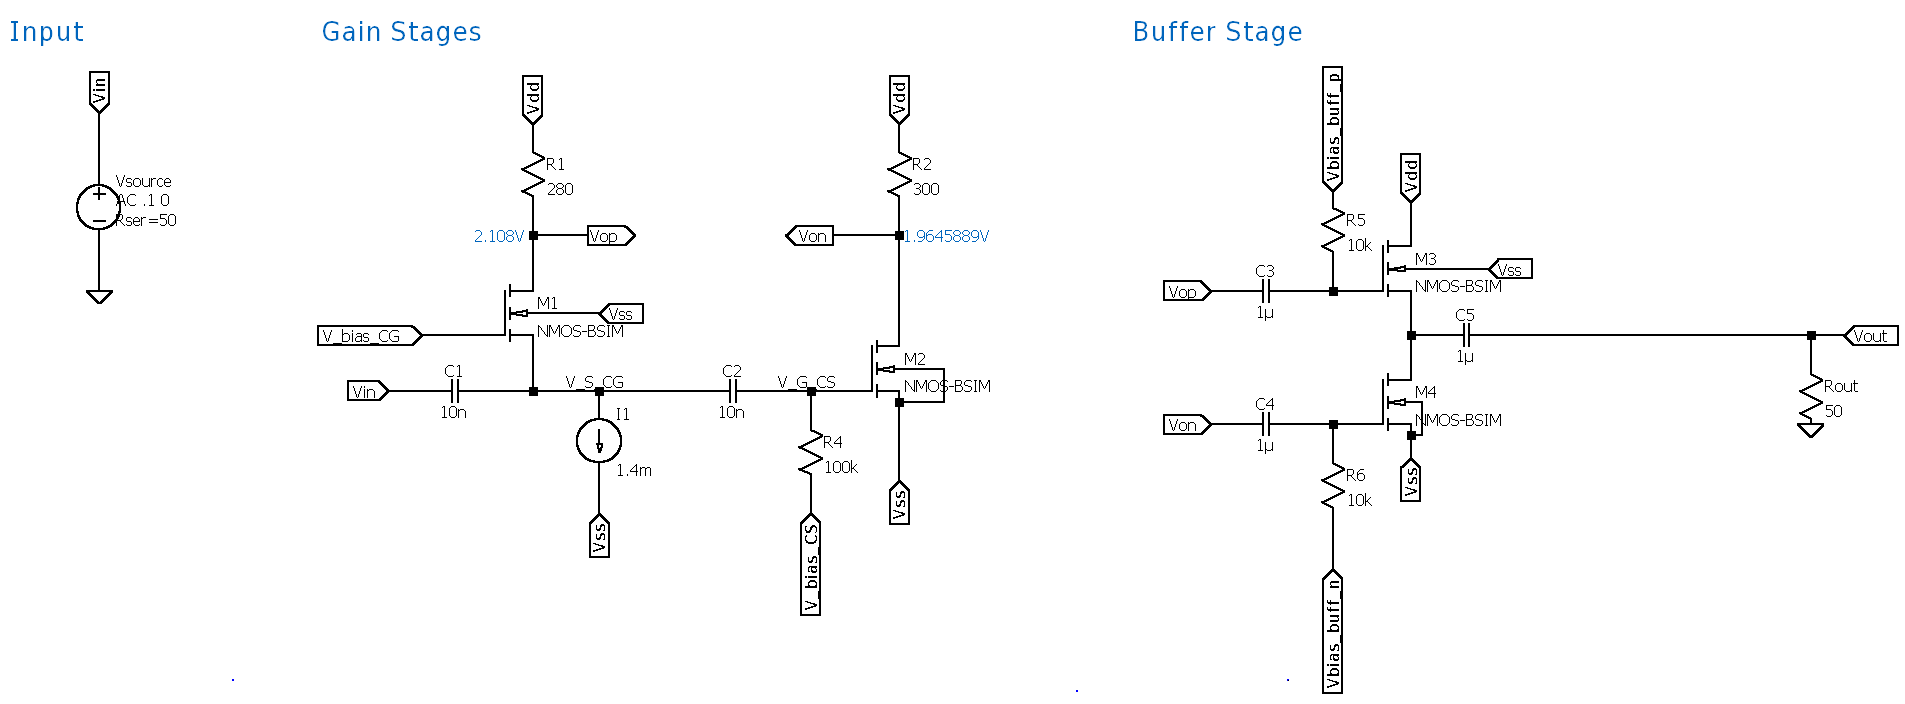
\includegraphics[width=0.9\textwidth]{Images/schem-LNA.png}
    \caption{Schematic of the gain stages in the proposed LNA architecture.}
    \label{fig:schem-lna}
\end{figure}

\subsection{Common Gate and Common Source combination gain stages}

The Low Noise Amplifier (LNA) implemented in this project adopts a wideband balun-LNA topology, which combines a common-gate (CG) stage and a common-source (CS) stage operating in parallel, as depicted in Figure \ref{fig:schem-gain-stages}. This configuration, proposed in \cite{Blaakmeer2008}, is particularly advantageous because it simultaneously enables input matching, output balancing, noise cancellation, and distortion suppression.

\begin{figure}[H]
    \centering
    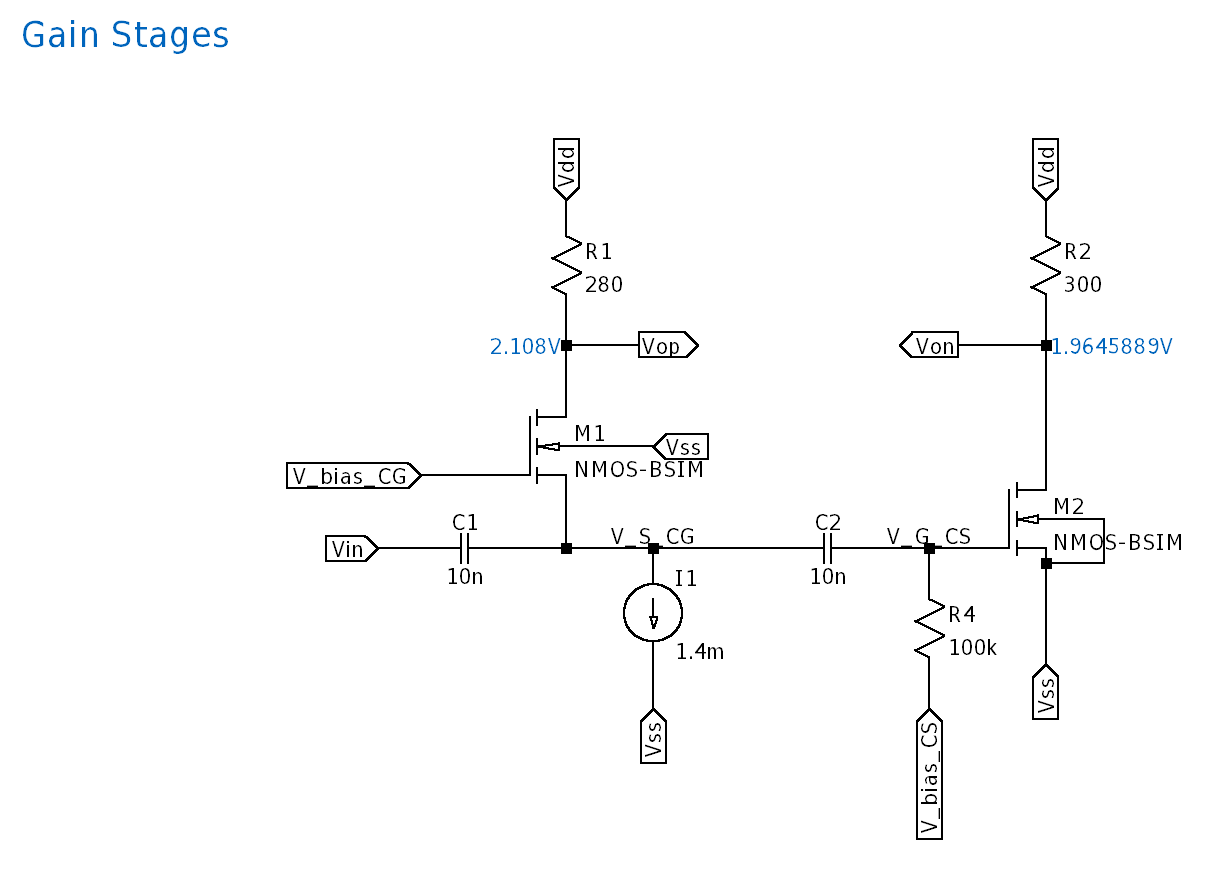
\includegraphics[width=0.8\textwidth]{Images/schem-GainStages.png}
    \caption{Schematic of the gain stages in the proposed LNA architecture.}
    \label{fig:schem-gain-stages}
\end{figure}

Analyzing the circuit in Figure \ref{fig:schem-gain-stages}, the input signal is amplified by two separate stages, the common-gate stage, where transistor M1 is used, and the common-source stage, where transistor M2 is used. The output is differential, with the positive signal taken from the drain of M1 and the negative signal from the drain of M2. ~The capacitors are used to couple the AC signals while blocking DC, ensuring that the DC biasing of the transistors does not affect the AC performance. 

\subsubsection{Common Gate Stage}

The CG stage, depicted in Figure \ref{fig:schem-cg}, provides a single-ended input with low input impedance, which makes it ideal for broadband input matching—specifically to $50 \si{\ohm}$ source impedance.

However, most receiver chains operate differentially, requiring a conversion from single-ended to differential signals. In this topology, the differential output is achieved by adding the CS stage in parallel with the CG stage, and balancing the gains of both paths with opposite polarities. This results in a balun behavior, allowing the circuit to simultaneously amplify and convert the input signal to differential form.

\begin{figure}[H]
    \centering
    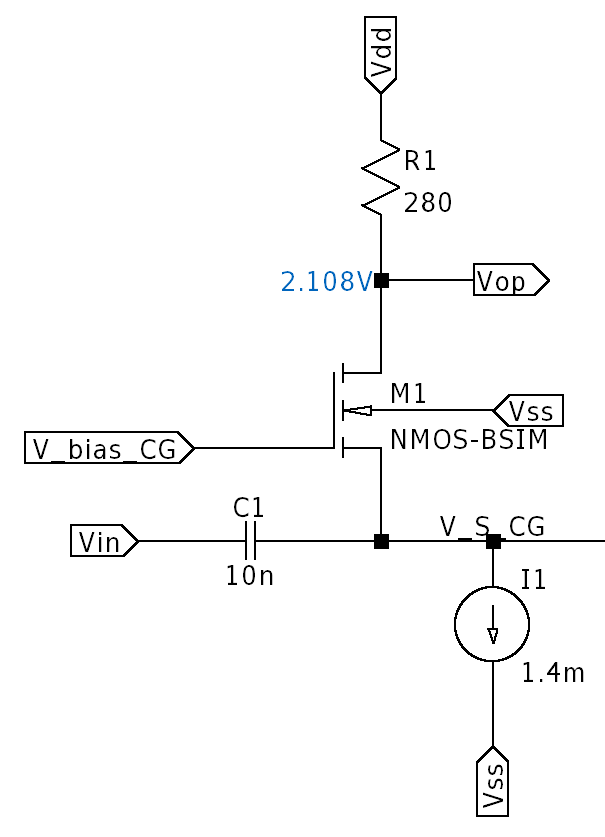
\includegraphics[width=0.3\textwidth]{Images/schem-CG.png}
    \caption{Schematic of the common-gate stage in the proposed LNA architecture.}
    \label{fig:schem-cg}
\end{figure}

\subsubsection{Common Source Stage}

The CS stage, shown in Figure \ref{fig:schem-cs}, provides a high input impedance and is typically used for voltage amplification. In this architecture, the CS stage is designed to operate in parallel with the CG stage, allowing for differential output while maintaining high gain. The CS stage also contributes to the overall noise figure and linearity of the LNA.

\begin{figure}[H]
    \centering
    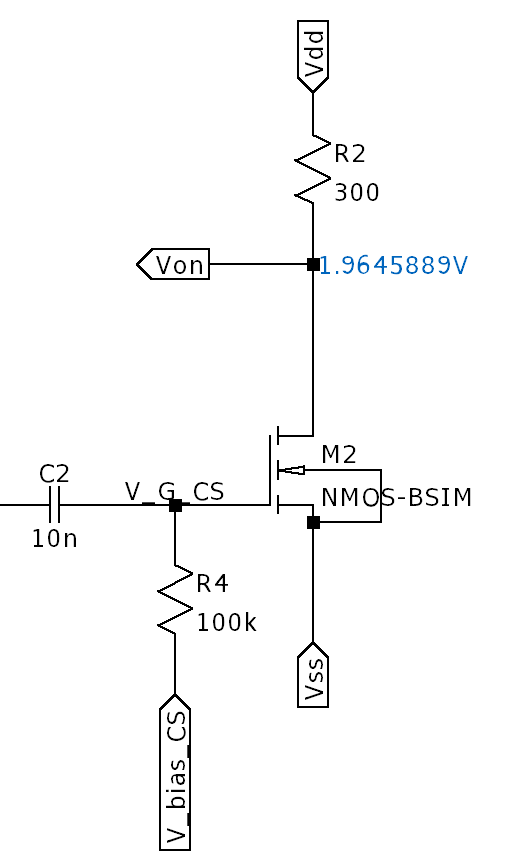
\includegraphics[width=0.3\textwidth]{Images/schem-CS.png}
    \caption{Schematic of the common-source stage in the proposed LNA architecture.}
    \label{fig:schem-cs}
\end{figure}

The noise produced by the CG transistor, mainly thermal noise, is a major contributor to the total noise figure in traditional designs. However, by carefully matching the gain of the CG and CS paths, the noise from the CG stage appears as a common-mode signal at the differential output and is effectively canceled. This cancellation occurs because the CG noise contributes identically to both outputs, while the CS stage contributes with opposite polarity. The result is a significantly reduced noise figure.

In addition to noise, the nonlinear distortion of the CG stage can also be canceled using this structure. When both paths have matched amplitude and phase but opposite sign, the nonlinear distortion generated by the CG stage also appears in-phase at both outputs and is canceled in the differential signal. As a result, the overall linearity is determined by the CS stage. The CS stage can then be optimized independently for linearity, allowing the design to achieve high dynamic range while maintaining wideband operation.

\subsection{Buffer Stage}

In the proposed LNA architecture, an output buffer, depicted in Figure \ref{fig:schem-buffer}, is included following the differential outputs of the common-gate and common-source stages. The buffer plays a crucial role in ensuring impedance matching, signal integrity, and measurement convenience.

\begin{figure}[H]
    \centering
    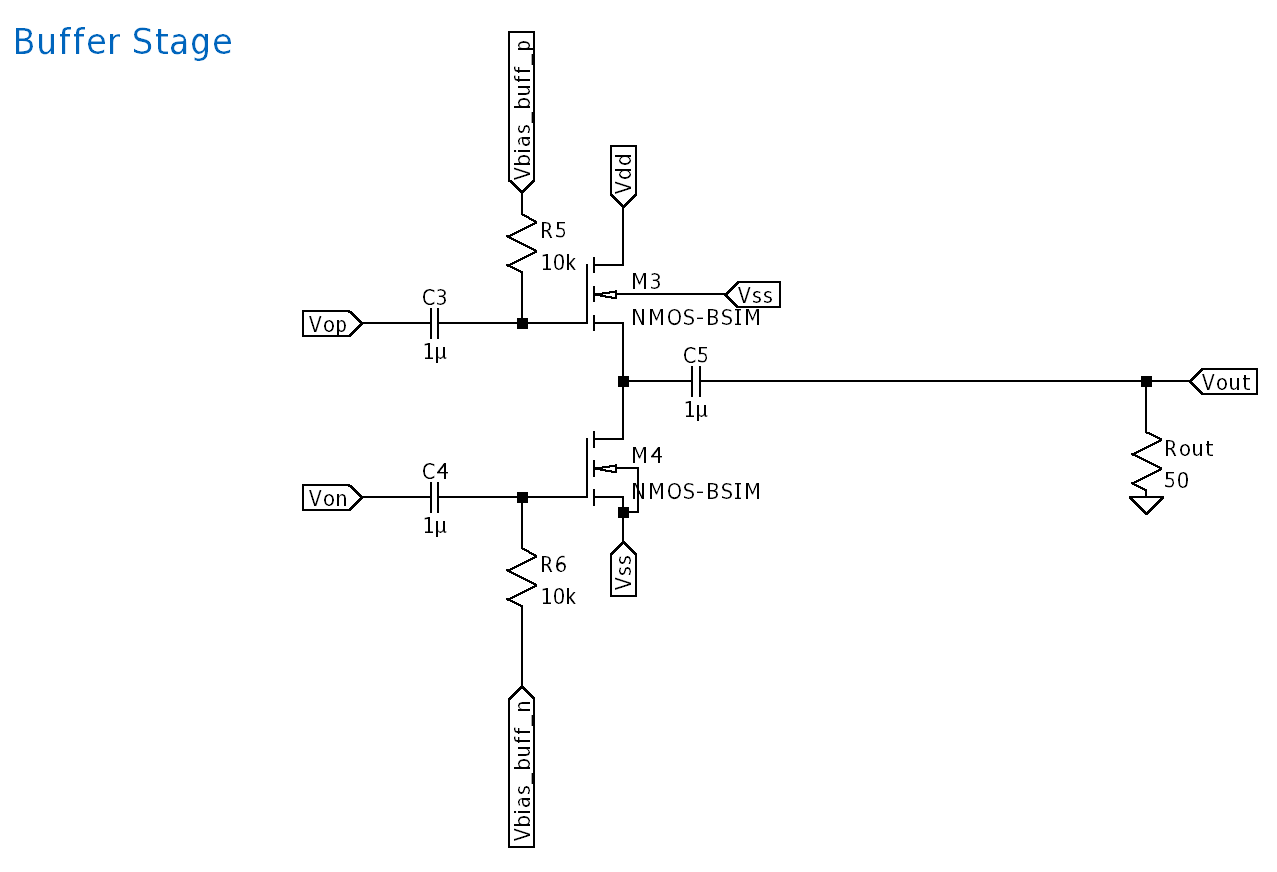
\includegraphics[width=0.8\textwidth]{Images/schem-Buffer.png}
    \caption{Schematic of the output buffer in the proposed LNA architecture.}
    \label{fig:schem-buffer}
\end{figure}

Analyzing the circuit the differential signal enters through the gates of both transistors, M3 in a common-drain configuration and M4 in a common-source configuration. Ideally, both configurations have a gain of 1, resulting in a single-ended output signal with a gain equal to the gain of the input signals. As in the previous circuit, the capacitors are used to couple the AC signals while blocking DC, ensuring that the DC biasing of the transistors does not affect the AC performance.

Firstly, in typical RF systems, the LNA output often needs to interface with $50 \si{\ohm}$ measurement equipment or subsequent stages (e.g., mixers) that have specific impedance requirements. The output buffer, provides a low output impedance while maintaining a high input impedance, effectively isolating the LNA core from the load. This allows the LNA to drive a standard $50 \si{\ohm}$ load without compromising its gain or linearity performance.

Secondly, the buffer helps to preserve the voltage gain achieved by the LNA. Without buffering, any mismatch or loading at the output could attenuate the signal and degrade performance. The buffer thus ensures that the full gain developed across the load devices is delivered to the output.

Thirdly, for testing and characterization purposes, the buffer is particularly important. In the measurement setup described in \cite{Bastos2014}, the output buffer is integrated with a balun/voltage combiner to enable single-ended measurements of the differential output. This facilitates direct connection to spectrum analyzers or vector network analyzers without the need for additional external components.

Finally, the inclusion of the buffer also contributes to robustness against variations in the following stage, whether in simulation or practical implementation, ensuring consistent performance across different configurations.